\section{Config\-Base Class Reference}
\label{classConfigBase}\index{ConfigBase@{ConfigBase}}
Inheritance diagram for Config\-Base::\begin{figure}[H]
\begin{center}
\leavevmode
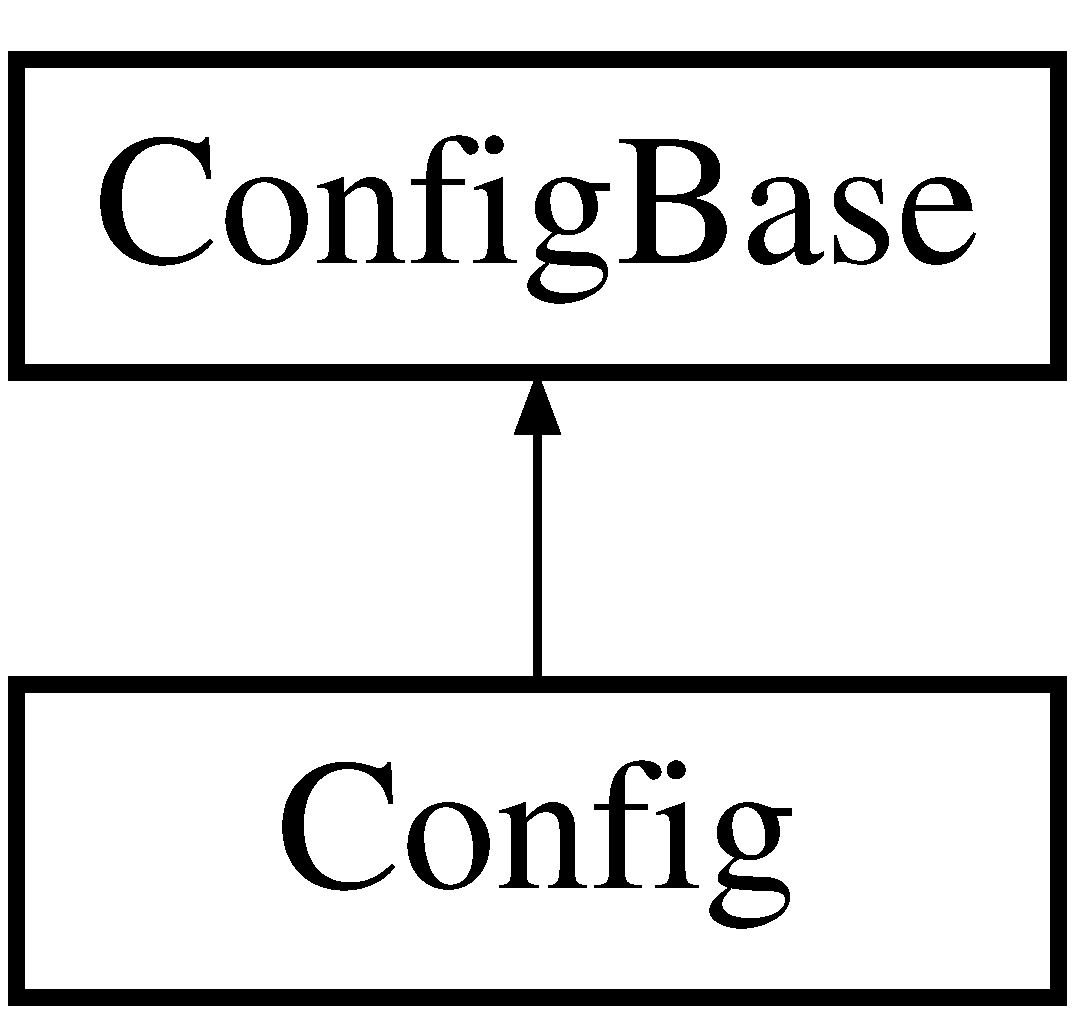
\includegraphics[height=2cm]{classConfigBase}
\end{center}
\end{figure}
\subsection*{Public Member Functions}
\begin{CompactItemize}
\item 
{\bf \_\-\_\-init\_\-\_\-} (name, def\_\-val)
\item 
{\bf update} (val)
\end{CompactItemize}


\subsection{Member Function Documentation}
\index{ConfigBase@{Config\-Base}!__init__@{\_\-\_\-init\_\-\_\-}}
\index{__init__@{\_\-\_\-init\_\-\_\-}!ConfigBase@{Config\-Base}}
\subsubsection{\setlength{\rightskip}{0pt plus 5cm}Config\-Base::\_\-\_\-init\_\-\_\- (name, def\_\-val)}\label{classConfigBase_ConfigBasea0}


\index{ConfigBase@{Config\-Base}!update@{update}}
\index{update@{update}!ConfigBase@{Config\-Base}}
\subsubsection{\setlength{\rightskip}{0pt plus 5cm}Config\-Base::update (val)}\label{classConfigBase_ConfigBasea1}




Reimplemented in {\bf Config} {\rm (p.\,\pageref{classConfig_Configa1})}.

The documentation for this class was generated from the following file:\begin{CompactItemize}
\item 
{\bf Config\-Admin.py}\end{CompactItemize}
